\documentclass{article}
\linespread{0.7}
\usepackage[a4paper, margin=3mm, landscape]{geometry}
\usepackage{multicol}
\usepackage{xcolor}
\usepackage{enumitem}
\usepackage{amsmath}
\usepackage{amsfonts}
\usepackage{listings}
\usepackage{soul}
\usepackage{graphicx}

\pdfinfo{
    /Title (GEC1010.pdf)
    /Creator (TeX)
    /Producer (pdfTeX 1.40.0)
    /Author (Vincent Pang)
    /Subject (GEC1010)
    /Keywords (GEC1010, nus, cheatsheet, pdf)
}

\graphicspath{ {./img/} }

\pagestyle{empty}
\setcounter{secnumdepth}{0}
\setlength{\columnseprule}{0.25pt}

% Redefine section commands to use less space
\makeatletter
\renewcommand{\section}{\@startsection{section}{1}{0mm}%
    {-1ex plus -.5ex minus -.2ex}%
    {0.5ex plus .2ex}%x
{\normalfont\large\bfseries}}
\renewcommand{\subsection}{\@startsection{subsection}{2}{0mm}%
    {-1explus -.5ex minus -.2ex}%
    {0.5ex plus .2ex}%
{\normalfont\normalsize\bfseries}}
\renewcommand{\subsubsection}{\@startsection{subsubsection}{3}{0mm}%
    {-1ex plus -.5ex minus -.2ex}%
    {1ex plus .2ex}%
{\normalfont\small\bfseries}}%
\makeatother

% Adjust spacing for all itemize/enumerate
\setlength{\leftmargini}{0.5cm}
\setlength{\leftmarginii}{0.5cm}
\setlist[itemize,1]{leftmargin=2mm,labelindent=1mm,labelsep=1mm}
\setlist[itemize,2]{leftmargin=2mm,labelindent=1mm,labelsep=1mm}

% Font
\renewcommand{\familydefault}{\sfdefault}

% Define colors for math formulas
\definecolor{myblue}{cmyk}{1,.72,0,.38}
\everymath\expandafter{\the\everymath \color{myblue}}

% Custom command for keywords
\definecolor{highlight}{RGB}{251,243,218}
\newcommand{\keyword}[2][]{\sethlcolor{highlight}\hl{\textbf{#2}} #1 - }
\newcommand{\ilkeyword}[1]{\sethlcolor{highlight}\hl{\textbf{#1}}}

% Define colors and style for code
\definecolor{codegreen}{rgb}{0,0.6,0}
\definecolor{codegray}{rgb}{0.5,0.5,0.5}
\definecolor{codered}{HTML}{CC241D}
\definecolor{backcolor}{rgb}{0.95,0.95,0.95}
\lstdefinestyle{codestyle}{
    backgroundcolor = \color{backcolor},
    commentstyle = \color{codegray},
    keywordstyle = \color{codered},
    stringstyle = \color{codegreen},
    basicstyle = \ttfamily,
    breakatwhitespace = false,
    showstringspaces = false,
    breaklines = true,
    showtabs = false,
    tabsize = 2
}
\lstset{style = codestyle}

% -----------------------------------------------------------------------
\begin{document}
\begin{multicols*}{4}
\footnotesize

% Title box
\begin{center}
    \fbox{
        \parbox{0.8\linewidth}{
            \centering \textcolor{black}{
                {\Large\textbf{GEC1010}} \\
                \normalsize{AY22/23 Sem 2}} \\
                {\footnotesize \textcolor{gray}{github.com/securespider}}
        }
    }
\end{center}
\section{01. Energy}
\subsection{By constant force}
work done by a force == force * displacement
\\$W = FS$
\subsection{Law of conservation of energy}
Energy can neither be created nor destroyed, it can only be transformed from one form to another
\subsection{Kinetic energy}
\keyword{linear motion}{$K=\dfrac{1}{2}mv^2$}\\
\keyword{angular motion}{$\dfrac{1}{2}I\omega^2$}
\begin{itemize}
	\item I = Moment of inertia of object (dependent on mass distribution of object)
	\item $\omega$ = angular velocity of the rotating object
	\begin{itemize}
		\item Rad/second
		\item $v = \omega * radius$
	\end{itemize}
\end{itemize}
\subsection{Gravitational potential energy}
$U = mgh$

\subsection{Power}
Rate of doing work or rate of consumption of energy\\
$P = \dfrac{\triangle W}{\triangle t}$\\
Work done, W, by a system in time t

\subsection{Requirements of an energy system}
\subsubsection{Energy resource}
\begin{itemize}
	\item Clean energy 
	\begin{itemize}
		\item Wind Energy
		\item \keyword{Hydro energy}{Come from river and dams}
		\item Ocean energy{Only refers to energy coming from ocean currents etc}
		\item Solar energy
		\item Biomass
		\item Non-Renewables:
		\item Geothermal
		\item Nuclear
	\end{itemize}
	\item Fossil fuels
	\begin{itemize}
		\item Coal
		\begin{itemize}
			\item Greater carbon content and more impurities - More carbon dioxide and greater air pollution
			\item Solid so difficulty in extraction, transportation and use
			
		\end{itemize}
		\item Natural Gas
		\begin{itemize}
			\item Cleaner alternative 
		\end{itemize}
		\item Oil
	\end{itemize}
\end{itemize}	
Problems
\begin{itemize}
	\item Unsustainable - reserves depleting
	\item Global warming - Enhanced greenhouse effect by earth atmosphere
	\item Greater absorption of long wavelength IR in earth's atmosphere
	\item Rising temperature anomaly from 1965-now by about 100mm
	\item Global sea level rising
	\begin{itemize}
		\item Thermal expansion of water
		\item Melting alpine glaciers and ice sheets
	\end{itemize}
	\item Earlier timing of spring events
	\item Poleward and upward shift in plant and animal species
\end{itemize}
Solution:\\
Clean energy
\begin{itemize}
	\item Replace existing supply of fossil fuels
	\item Use energy more efficiently and judiciously minimizing environmental pollution
\end{itemize}
\subsubsection{High power}
\subsubsection{High energy conversion efficiency}
\subsection{Singapore}
Singapore uses LNG primarily (95\%) piped from indonesia and malaysia\\
Switching to \textbf{solar} and biofuels to reduce reliance
\subsubsection{Energy conservation}
\begin{itemize}
	\item Outdoor LED initative
	\item Electric car sharing
\end{itemize}

% -----------------------------------------------------------------------

\section{02. Fundamentals of thermal energy}
$Q=mc\triangle T$
\begin{description}
	\item[Q]{Heat energy supplied}
	\item[m]{mass}
	\item[c]{Specific heat capacity of material}
	\item[T]{temperature change resulting from heat energy}
\end{description}
$Q=mL$
\begin{description}
	\item[Q]{Heat energy supplied}
	\item[m]{mass}
	\item[L]{Specific latent heat of vaporization/fusion}
\end{description}

\subsection{Types}
\begin{itemize}
	\item Conduction
	\begin{itemize}
		\item Dominant in solids
		\item No bulk motion of matter
		\item Heat flows from region of high temperature to region of low temperature
	\end{itemize}
	\item Convection
	\begin{itemize}
		\item Dominant in fluids (liquid and gases)
		\item Works by circulating fluids and thermal expansion properties of materials
		\item Cold fluids sink, warm fluid rise
	\end{itemize}
	\item Radiation
	\begin{itemize}
		\item Uneven, black bodies absorb/emit better
	\end{itemize}
\end{itemize}

\subsection{Stefan Boltzmann Law}
Power of black body radiation\\
$P = \epsilon\sigma T_0^4$
\begin{enumerate}
	\item[P]{Energy absorbed per unit second per unit area via radiation}
	\item[$\epsilon$]{Emissivity of surface(lies between 0-1)}
	\item[$\sigma$]{$5.67*10^{-8}$ = Stefan Boltzmann constant}
\end{enumerate}
\subsection{First law of thermodynamics}
Difference between the heat absorbed Q and the work done W on object is equal to change in internal energy of the thermodynamic system\\
$Q-W=\triangle U$

\subsection{Steam based thermal power plant}
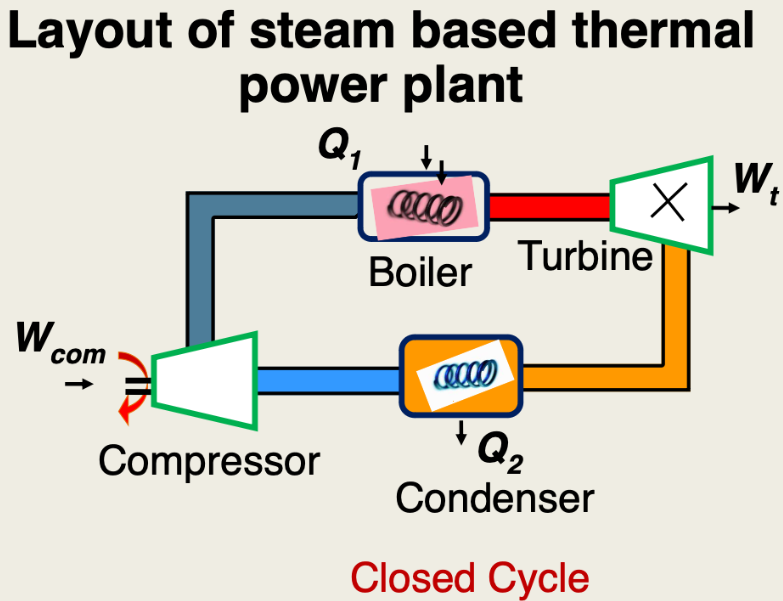
\includegraphics[scale=0.25]{boiler_system}\\
Key stages
\begin{description}
	\item[Compression]{Work done on system to compress cold water to high pressure}
	\item[Boiling]{Heat added to the system to convert cold water into steam}
	\item[Turbine rotation]{Work $W_{t}$ done by the system on turbine blades}
	\item[Condensation]{Heat lost from the system to the environment in converting steam back to cold water}
\end{description}
\begin{itemize}
	\item Working fluid have the same amount of energy U as it had in the beginning of the cycle
%	\item Net work done by the system = $W_t - W_{com}$
	\item Net heat absorbed = $Q_{2} - Q_{2}$
\end{itemize}
Efficiency of cycle is given by \\
$\eta = \dfrac{Net~output~work}{heat~input} = \dfrac{W_{t} - W_{com}}{Q_{1}} = \dfrac{Q_{1}-Q_{2}}{Q_{1}} = 1-\dfrac{Q_{2}}{Q_{1}}$

\subsection{Rankine cycle}
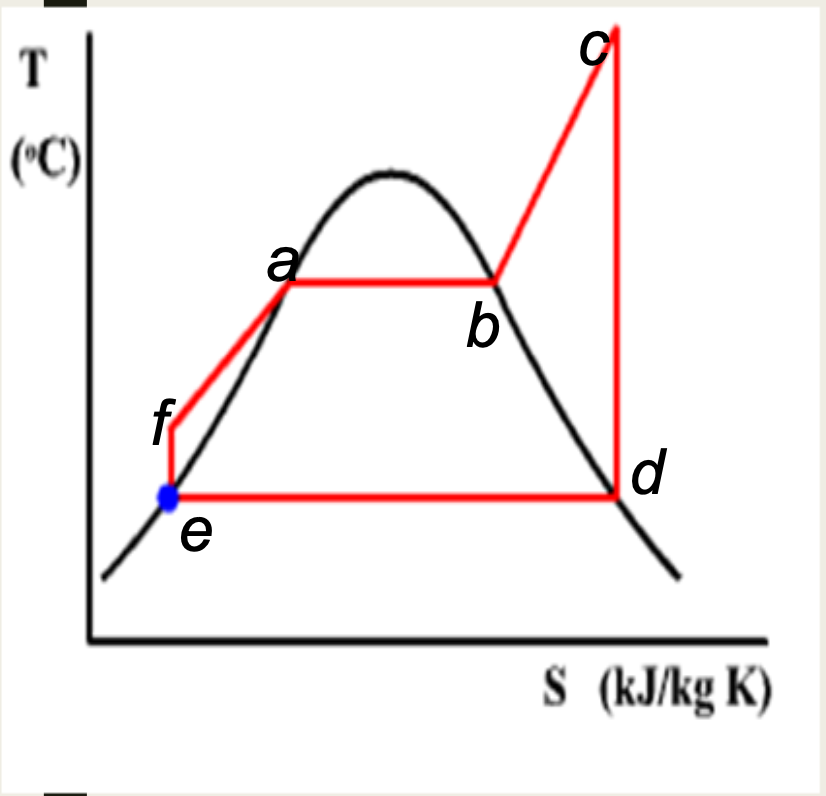
\includegraphics[scale=0.3]{rankine_cycle}\\
Steam power plant energy generation (Temperature - entropy graph)
\begin{itemize}
	\item EF - Compressor increases the pressure of water
	\item FA - Economiser, Water heated at high pressure until it boils
	\item AB - Evaporator, 2 phase mixture of water and steam is heated at constant pressure until all water converted to dry steam
	\item BC - Superheater, Dry steam heated at constant pressure in superheater
	\item CD - Dry steam enter turbine at high pressure and rotate the turbine 
	\item DE - Steam converted to water
	\begin{itemize}
		\item Problem: Unable to completely eliminate the formation of water droplets @ CD
		\item Solution: Reheat the steam at CD to rotate the turbine again
		\item Temperature is raised again, leading to greater efficiency
		\item Achieve 40\% efficiency
		\item Cannot go beyond 650c to prevent metal fatigue
	\end{itemize}
\end{itemize}
\subsection{Brayton cycle}
Use gas instead of water leading to no worry of water droplets and can go higher temperatures


% -----------------------------------------------------------------------
\section{03. Wind energy}
\subsection{How wind forms}
\subsubsection{Dominant}
\begin{itemize}
	\item \keyword{Coriolis Effect}{Sideward component of wind due to earth rotation}
	\item \keyword{Solar radiation}{Warm air rise up in the equator leading to difference in densities}
\end{itemize}

\subsubsection{Other factors}
\begin{itemize}
	\item Ocean
	\begin{itemize}
		\item Water absorbs/releases heat slower than land
		\item Day: Water less hot, sea -\> land
		\item Night: Water hotter, land -\> sea
	\end{itemize}
	\item Surface friction
	\item Eddy motion
	\item Seasonal effects	
\end{itemize}

\subsection{Power of wind}
$P=\dfrac{1}{2}\rho Au^3$\\
Wind speed affected by height of the turbines
\begin{itemize}
	\item Wind speed rises proportionally to 7th root of altitude
\end{itemize}
\subsection{Wind turbines}
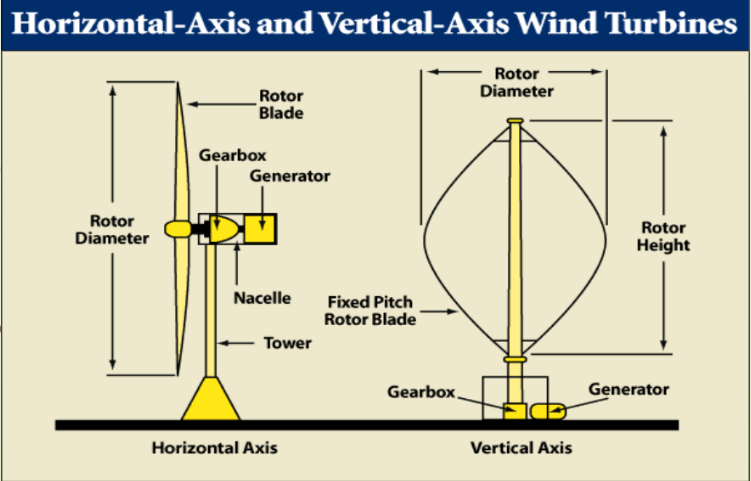
\includegraphics[scale=0.3]{wind-turbine}
\begin{itemize}
	\item \keyword{Yaw control}{Orientates the nacelle in direction of incident wind}
	\begin{itemize}
		\item Note: Better for rotor to face the wind
		\item Less wind shadowing effect
		\item Blades flex less
		\item Less fatigue in the blades
	\end{itemize}
\end{itemize}
\subsection{Forces}
\begin{description}
	\item[Drag]{Net force in direction of wind}
	\item[Lift]{Net force perpendicular to wind}
\end{description}
\subsection{Blades}
Turbines cause turbulence for surrounding blades so cannot have too many blades\\
\keyword{Tip Speed Ratio (TSR)}{$\dfrac{Speed~of~rotation~of~outer~tip~of~blade}{incident~wind~speed}$}\\
\keyword{Betz limit}{Maximum theoretical efficiency of rotor}\\
\keyword{Capacity factor}{$\dfrac{yield}{rated~power}$}\\
Dependent on wind speed

\subsection{Offshore vs Onshore}
\begin{itemize}
	\item[+] Wind speed is faster offshore
	\item[+] Less obtrusive
	\item[+] Bigger in size
	\item[+] CF higher
	\item[-] Harder to maintain cus in the sea (But easier to build because transportation over water easier)
	\item[-] Might spoil faster due to seawater
\end{itemize}

% -----------------------------------------------------------------------
\section{04a. Solar Power}
Renewable form of energy with $3.9x10^{26}W$\\
Only half reach surface of earth
\subsection{Types of systems}
\begin{itemize}
	\item \keyword{Passive}{Uses no external power}
	\begin{itemize}
		\item Allows fluid heated by the sun to circulate by natural means
	\end{itemize}
	\item \keyword{Active} {Solar heated fluid is circulated by a fan or pump}
\end{itemize}
\subsection{Solar fluid collectors}
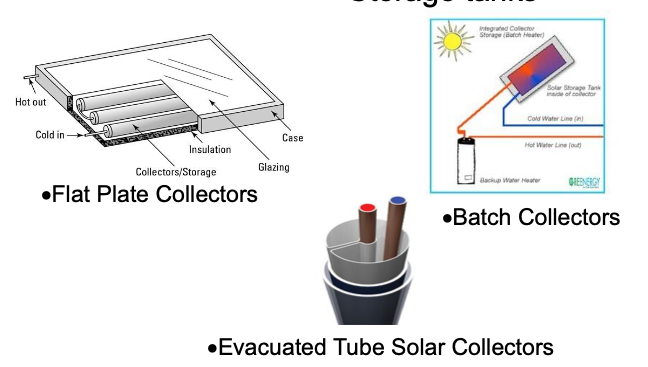
\includegraphics[scale=0.3]{solar-collectors}
\subsection{Passive space heating system}
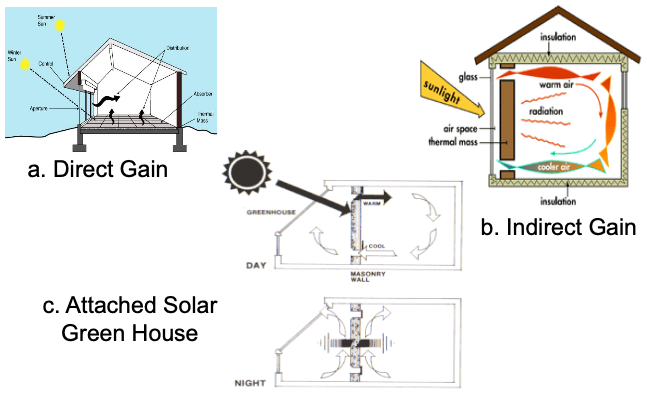
\includegraphics[scale=0.25]{passive-heating}
\subsubsection{Trombe wall}
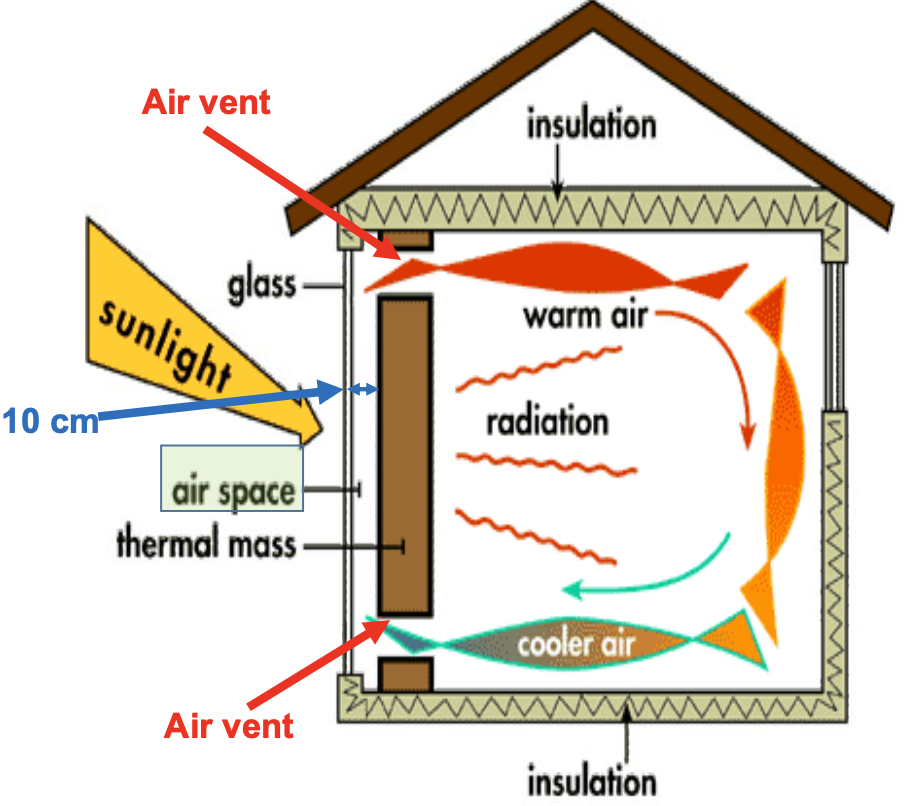
\includegraphics[scale=0.3]{trombe-wall}
\subsection{Principles of passive cooling}
\begin{itemize}
	\item Minimise solar heat gain
	\begin{itemize}
		\item Increase building mass
		\item Increase thermal protection
		\item REflective coating on exposed surface
		\item shading device
		\item Air tightness in building
	\end{itemize}
	\item Remove unwanted heat
	\begin{itemize}
		\item Evaporative cooling
		\item Nocturnal ventilation
		\item Thermo-active ceiling
	\end{itemize}
\end{itemize}
\subsection{Solar power energy}
Using the heat by the sun to drive rankine cycle
\begin{itemize}
	\item using mirrors to focus sun light into a tower to heat molten salt
	\item Run focus pipes surrounded my mirrors to heat the fluid in the pipes to be used to generate heat
\end{itemize}

\section{04b. Solar Photovoltaics}
$E=hf=\dfrac{hc}{\lambda} |$
$h=6.63*10^{-34},c=3*10^{8}$
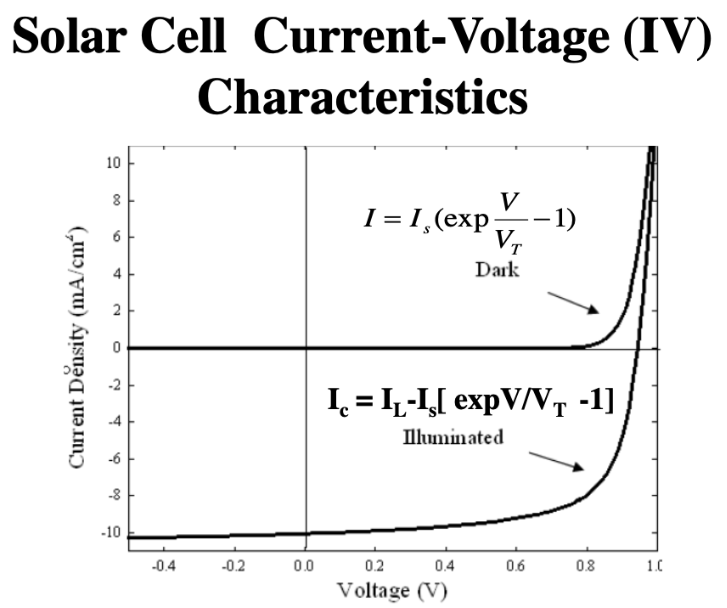
\includegraphics[scale=0.2]{i-v-characteristic}\\
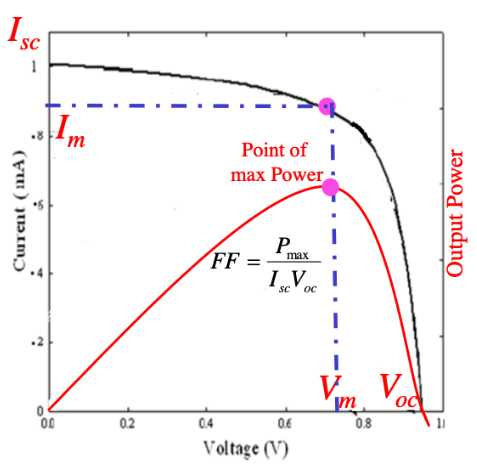
\includegraphics[scale=0.23]{fill-factor}
\subsection{Band gap}
Minimum energy that is required to excite an electron up to a state in the conduction band where it can participate in conduction\\
Higher short circuit current -\> lower bandgap
\subsection{Silicon}
Types
\begin{itemize}
	\item Polycrystalline
	\item Crystalline
	\item Amorphous
\end{itemize}
\subsubsection{Mechanism}
Transfer of electrons from n-types and p-types to maintain electric potential
\begin{itemize}
	\item \keyword{N-type}{Electron rich (conduct via electrons)}
	\begin{itemize}
		\item Doped with elements with more valence electrons (P)
		\item Cathode (negative terminal where current flows into when illuminated)
	\end{itemize}
	\item \keyword{P-type}{Electron deficient (conduct via holes)}
	\begin{itemize}
		\item Doped with elements with less valence electrons (Al)
		\item Anode (postive terminal where current flows out of when illuminated)
	\end{itemize}
	\item Pink arrow denotes conventional current
\end{itemize}
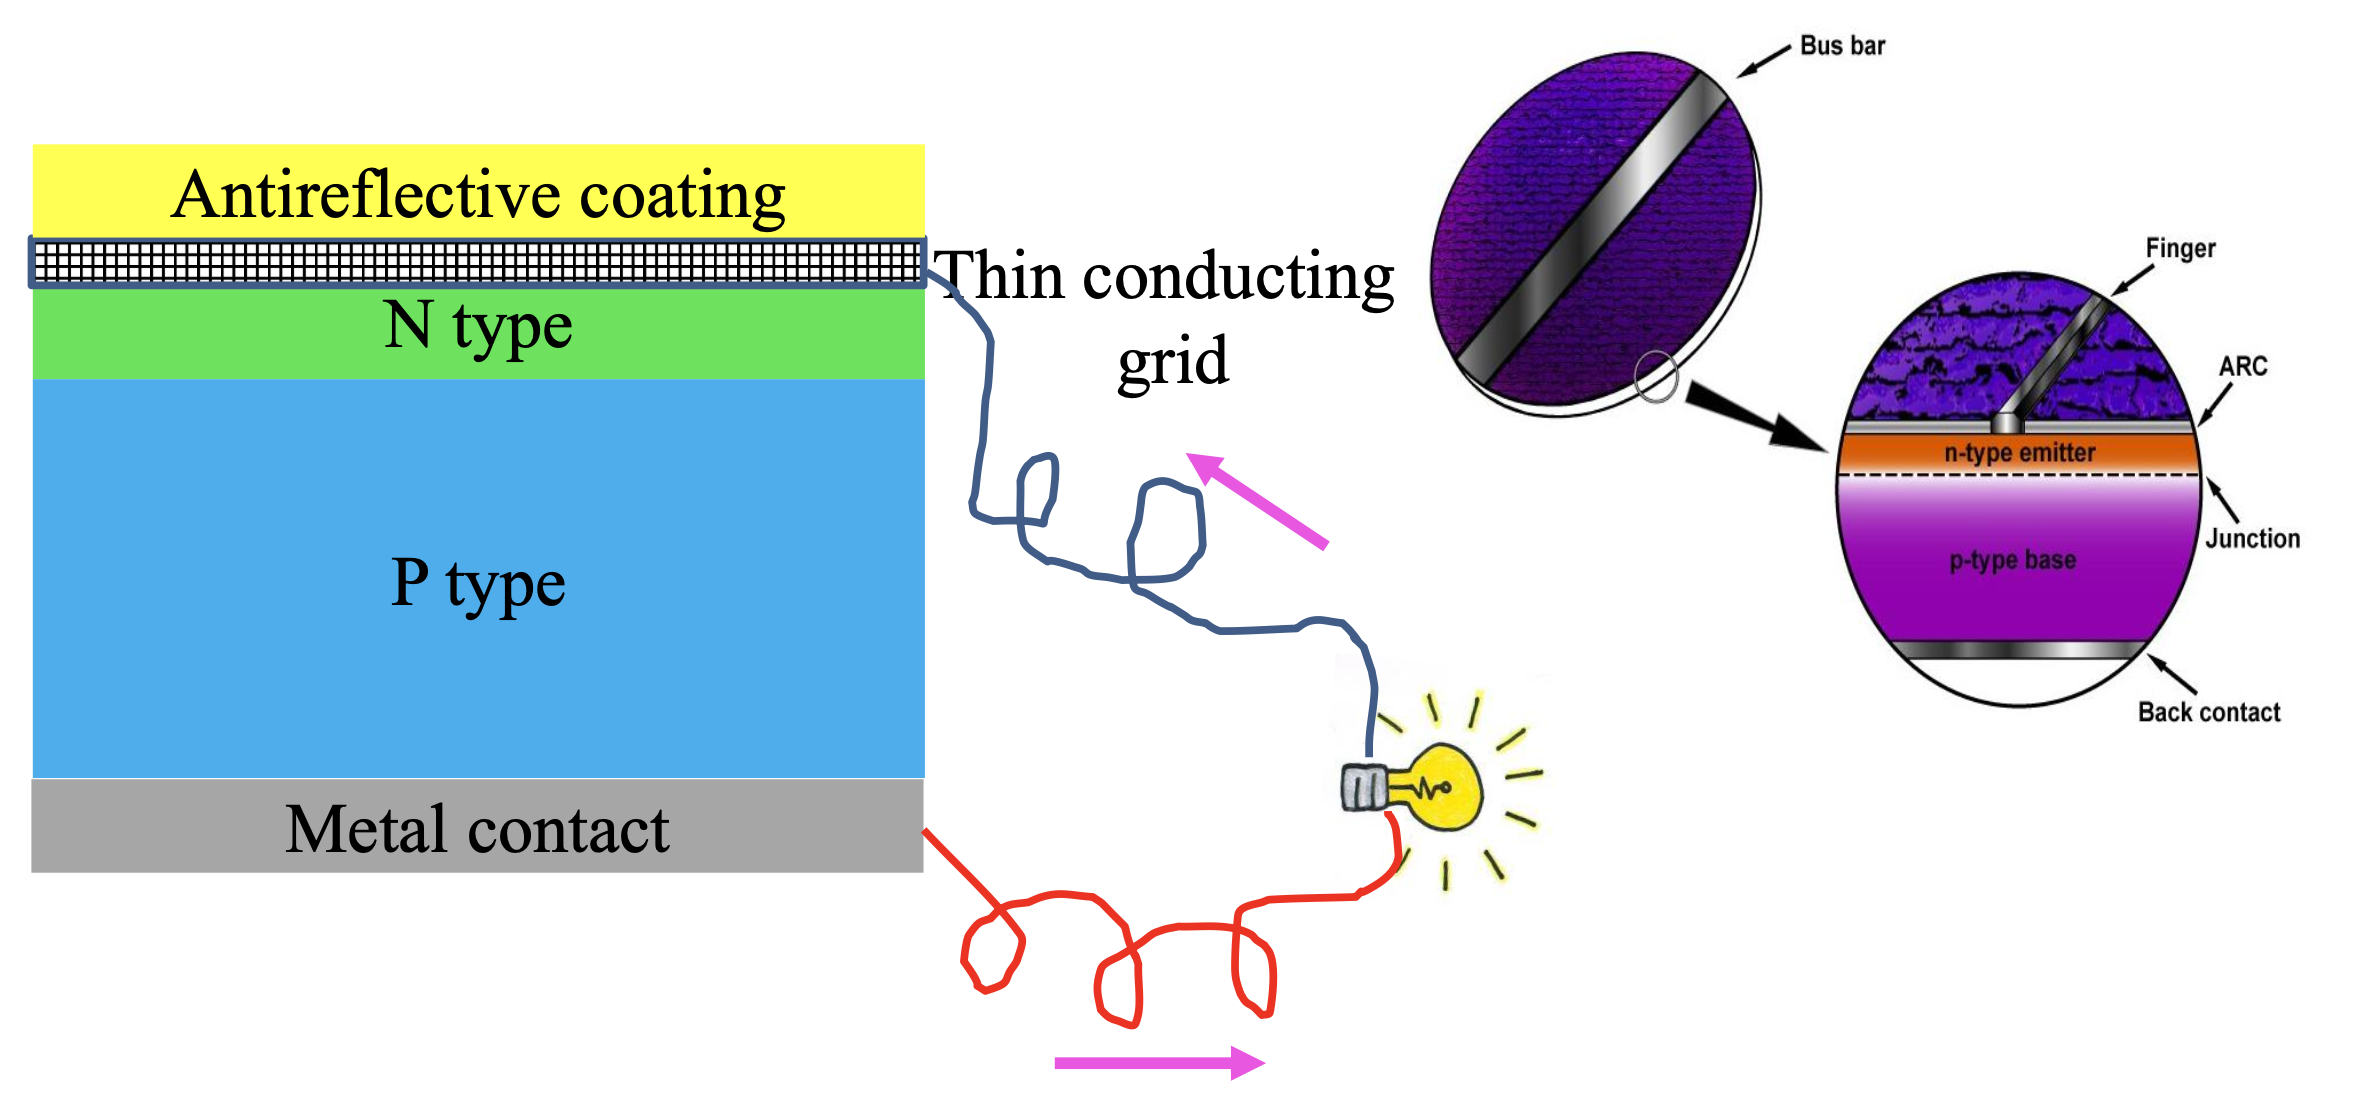
\includegraphics[scale=0.18]{solar-cell}
\subsubsection{Efficiency}
\begin{itemize}
	\item 23\% of photons has less energy than bandgap
	\item 30\% heat energy and 10\% loss from electron hole-pair recombination
	\item Increase efficiency by using anti-reflective coating
	\item Smaller bandgap -\> greater photocurrent but decrease output voltage (optimum 1.4eV gap)
\end{itemize}

% -----------------------------------------------------------------------
% -----------------------------------------------------------------------

\section{05a. Hydro power}
\subsection{Ocean vs River}
River
\begin{enumerate}
	\item Hydroelectricity
\end{enumerate}
Ocean
\begin{enumerate}
	\item Tidal power
	\item Wave power
	\item Ocean thermal
\end{enumerate}
\subsection{Water wheels}
\subsubsection{Water mills}
\begin{itemize}
	\item Ancient application for replacing physical labour
	\item Replaced with water turbines for energy generation
\end{itemize}
Types of water wheels\\
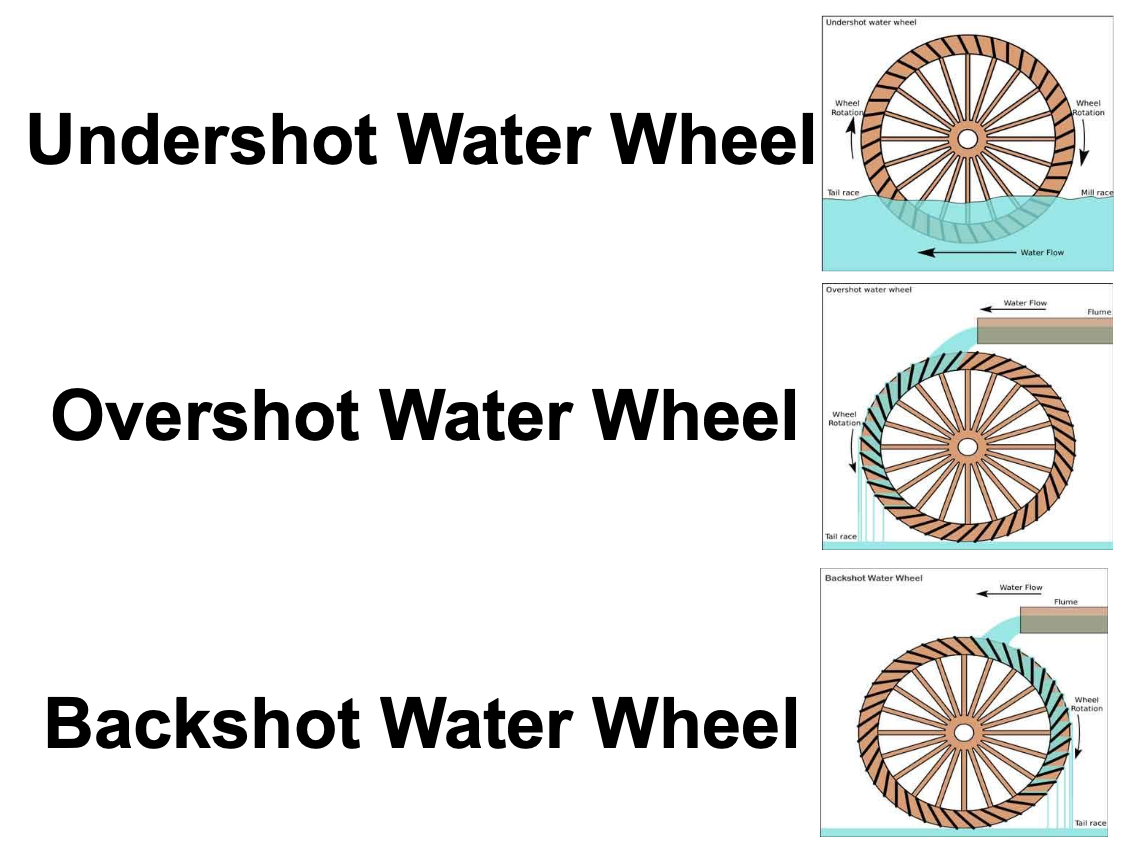
\includegraphics[scale=0.3]{water-wheels}
\begin{itemize}
	\item Undershot
	\begin{itemize}
		\item Vertically mounted with water flowing at the bottom of the wheel
		\item Cheapest and least efficient
	\end{itemize}
	\item Overshot
	\begin{itemize}
		\item Falling water on the top of the wheel in direction of rotation
		\item Use all water flow for power production 
		\item Does not require rapid flow of water
		\item Uses the difference in weight between the 2 sides of the wheel to turn
	\end{itemize}
	\item Backshot
	\begin{itemize}
		\item Introduced behind the apex of the wheel
		\item Water flows opposite the direction of rotation
		\item Continues to function even when water in wheel put rises beyond height of axle
		\item Technique useful for streams that experience extreme seasonal variations in flow
	\end{itemize}
\end{itemize}

\subsection{Types of Hydro Power}
\begin{itemize}
	\item Dam based
	\item Run of the river plants(diversion)
	\item Pumped storage technology
	\item Damless hydro power
\end{itemize}
\subsubsection{Principles of power generation}
Production of electricity by using gravitational force of falling water\\
$P=\eta\rho ghQ$\\
$\eta$ = efficiency, $\rho$ = density of water, Q = Volume of water flowing per second on turbine, h = Vertical distance between turbine and water surface

\subsubsection{Types of water turbines}
Impulse
\begin{itemize}
	\item Simpler and cheaper design -\> Easier to fabricate and maintain
	\item Needs higher head height
	\item Higher volume flow rate
	\item Greater tolerance of sand and other particles in water
	\item Better access to working parts
\end{itemize}
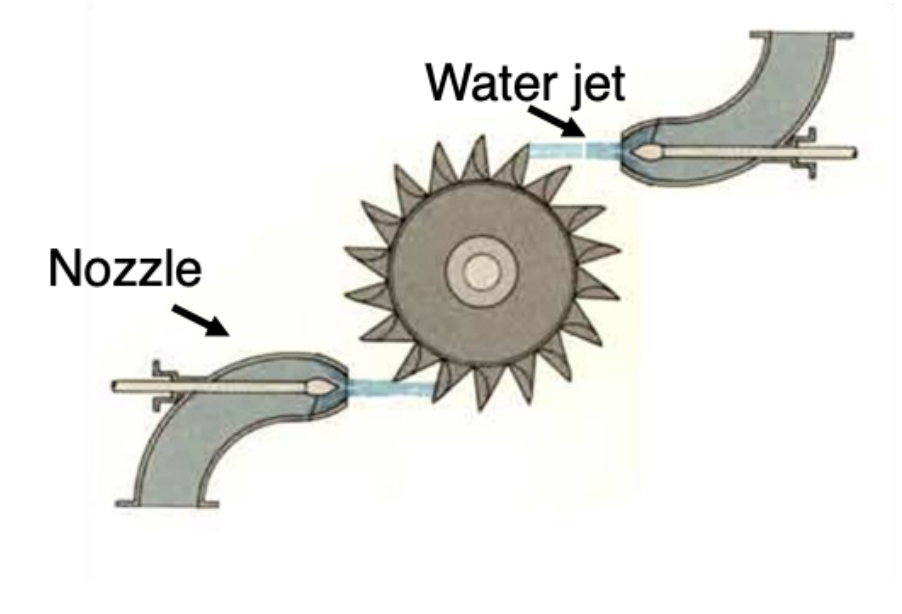
\includegraphics[scale=0.3]{pelton-turbine}\\
Reaction
\begin{itemize}
	\item Rotating element in reaction turbine enclosed in pressure casing to generate energy
	\item Rotates faster than impulse turbines given same head and flow conditions
	\item More expensive 
\end{itemize}
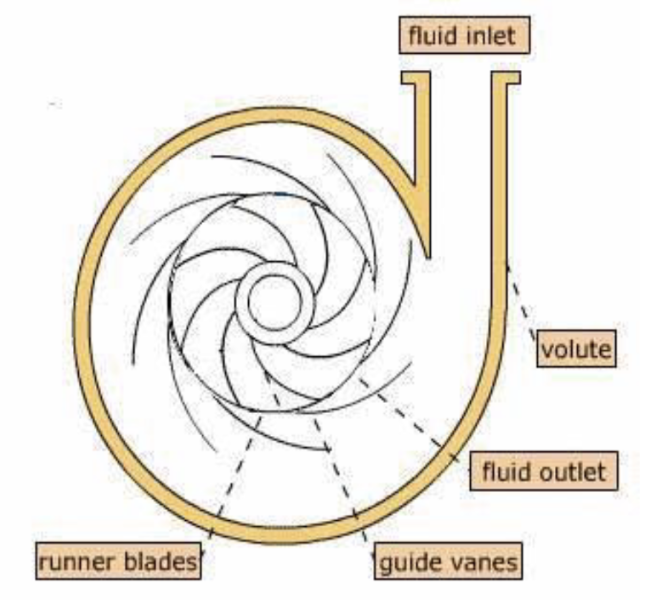
\includegraphics[scale=0.4]{reaction-turbine}

\subsection{Run of the river}
\begin{itemize}
	\item Low-level diversion weir/stream bed instead of dam
	\item Located on fast flowing, non seasonal stream 
	\item Minimize impact on environment
\end{itemize}

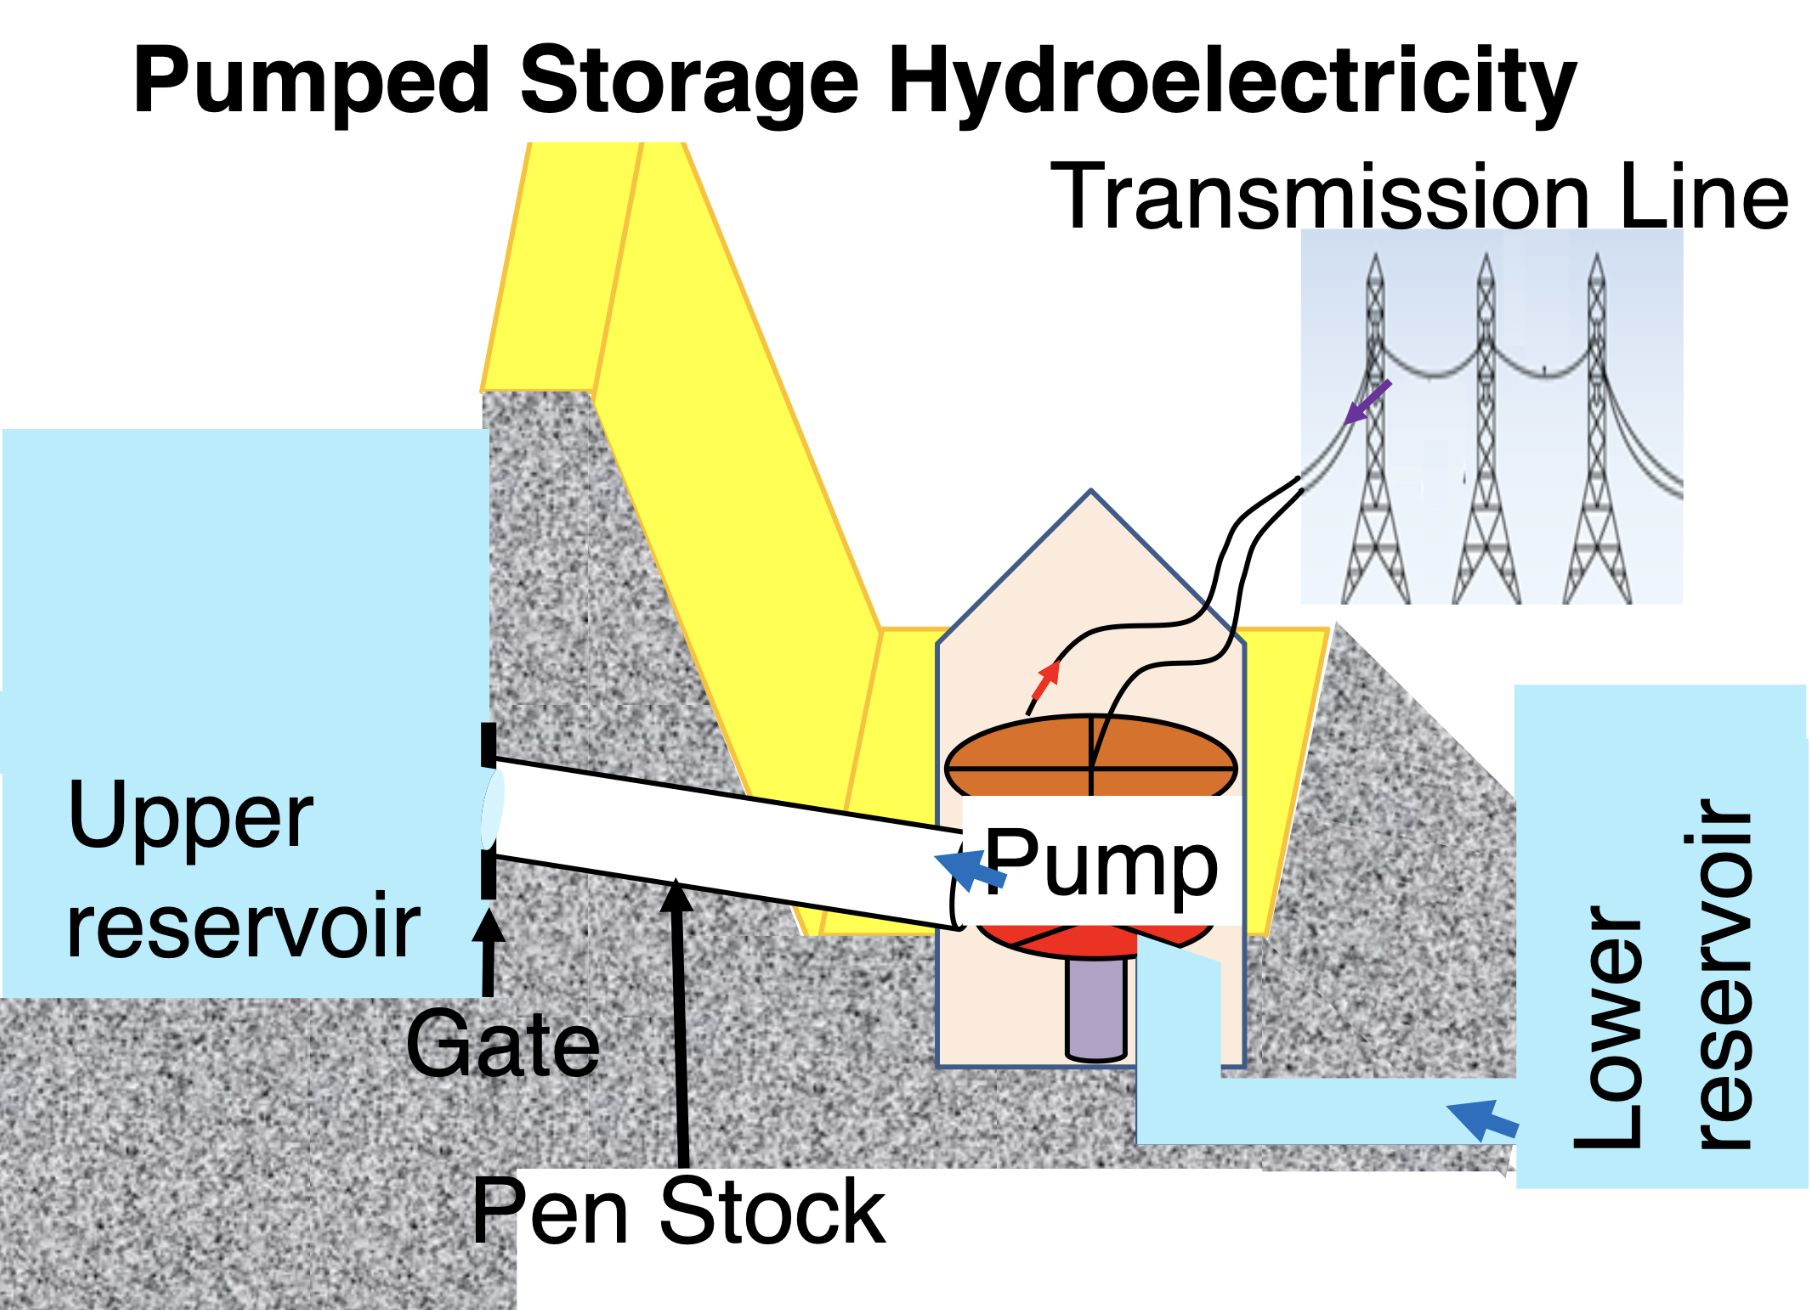
\includegraphics[scale=0.2]{pumped-storage}
\subsection{Pumped storage hydro}
\begin{itemize}
	\item Load balancing by storing energy pumped from lower elevation reservoir up
	\item Low cost off peak power to run pumps and released when high demand
	\item Net consumer of energy but largest capacity form of grid energy storage	
\end{itemize}

\subsection{Damless hydro}
\begin{itemize}
	\item Little to no maintenance
	\item Low initial setup cost and environmental impact
	\begin{itemize}
		\item No risk of flash flooding/dam-related accidents
		\item No silt accumulation and fish ladders
	\end{itemize}
\end{itemize}

\subsection{Advantage of hydroelectric}
\begin{itemize}
	\item Clean renewable energy (Low level of greenhouse gases)
	\item Low operating cost and highly automated
	\item Plant life is long $\approx$ 40 years
	\item Available on demand as flow rate is controlled
\end{itemize}
\subsection{Problems with hydroelectric}
\begin{itemize}
	\item Capital cost is high and payback time is long
	\item Social issues with displacement of population
	\item Environmental impact (Diversion of water)
\end{itemize}

\section{05b. Ocean Power}
\begin{enumerate}
	\item Tidal energy
	\begin{itemize}
		\item Gravitational field of sun and moon
	\end{itemize}
	\item Ocean wave energy
	\item Ocean thermal energy
\end{enumerate}
\subsection{Tidal energy}
\begin{itemize}
	\item Derived from gravitational interaction between Earth and Moon
	\item Bulge on opposite side due to earth's attraction
	\item Low and high tide occuring simultaneously at 2 places with longitudes differing by 90
	\item Interval between high tides approximately 12h
	\item \keyword{tidal range}{Difference between height of high and low tides}
	\item \keyword{Spring tides}{Moon and sun align leading to unusually high tides}
	\item \keyword{Neap tides}{Moon perpendicular to sun wrt earth leading to weak tides}
\end{itemize}
\subsubsection{Tidal barrage}
\begin{itemize}
	\item Dam built across river estuary
	\item High tides: Seawater flows into reservoir of barrage and rotate the turbine blades
	\item Low tides: Seawater stored in barrage is allowed to flow back out into sea turning turbines
	\item Output power $P=\dfrac{\eta\rho g A h^2}{T}$
	\begin{itemize}
		\item T is tidal period (time interval between 2 successive high tides)
	\end{itemize}
\end{itemize}
\subsubsection{Advantages}
\begin{itemize}
	\item Free, reliable and green (low maintenance)
	\item Turbines are cheap and do not cause large environmental impact
\end{itemize}
\subsubsection{Disadvantages}
\begin{itemize}
	\item Only provides power for about 10 hours each day (when tides moving)
	\item Tidal barrage sites are limited
	\item Fish ladders have to be installed and total cost is expensive
\end{itemize}
\subsection{Ocean current and waves}
\begin{itemize}
	\item Horizontal movement of seawater in the ocean
	\item Factors affecting:
	\begin{itemize}
		\item Intensity of solar radiation
		\begin{itemize}
			\item Fast moving air from sea surface to land
			\item Water dragged along the wind
		\end{itemize}
		\item Air temperature
		\item Wind speed and direction
		\item Gravitational pull of sun and moon
	\end{itemize}
	\item Moving up and down in circles
\end{itemize}
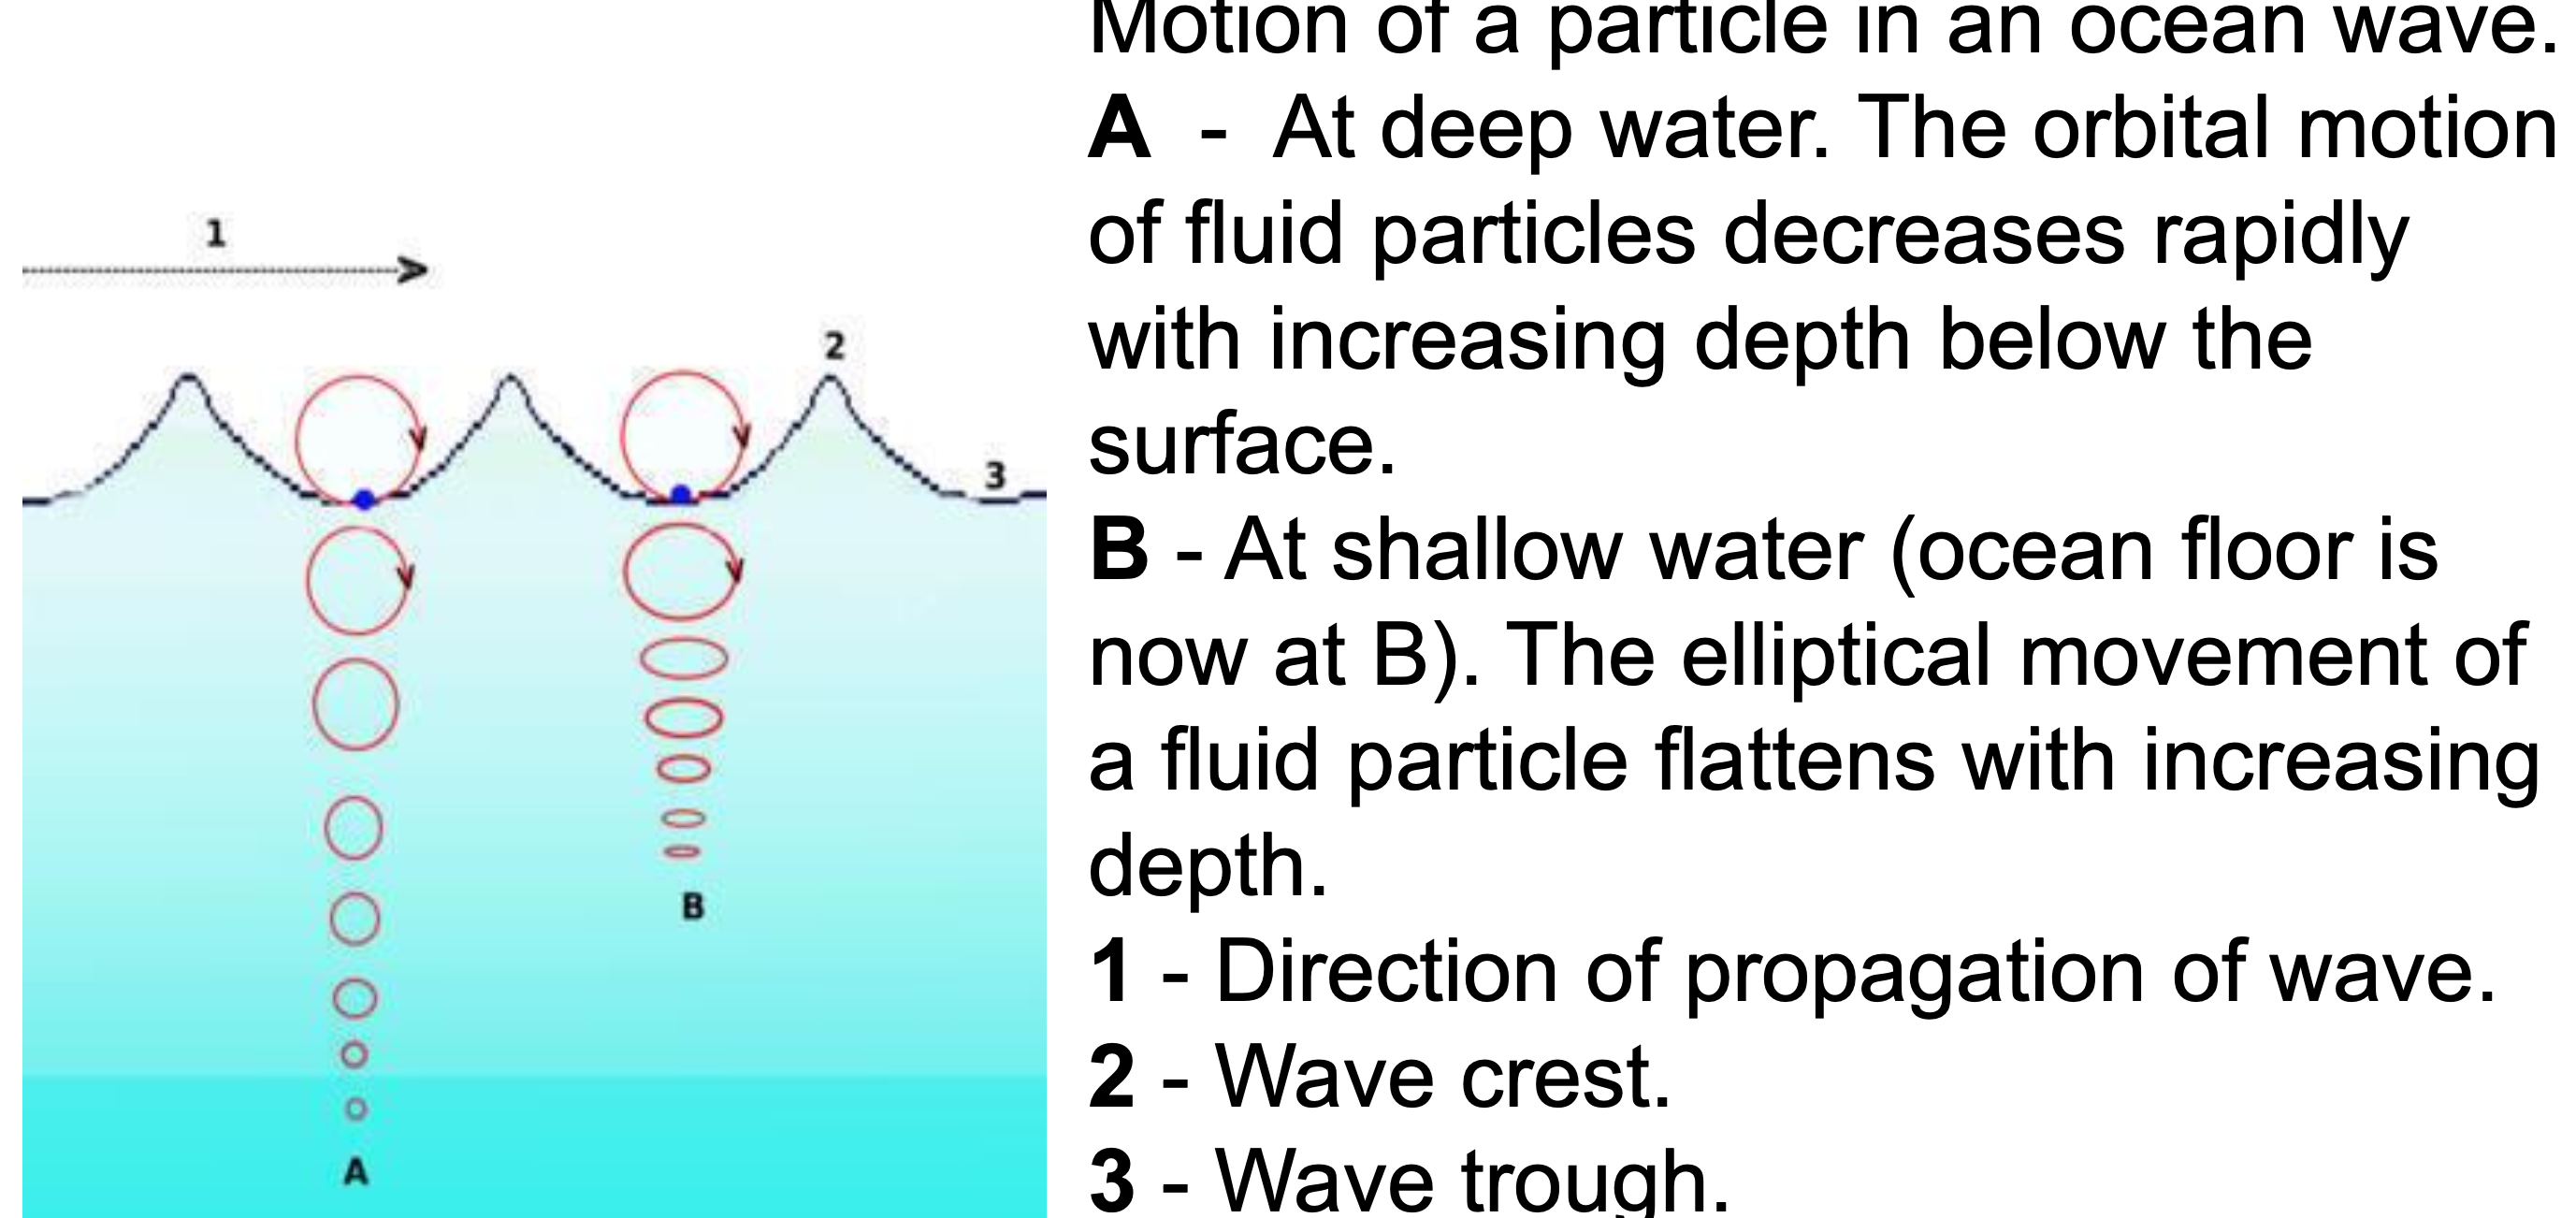
\includegraphics[scale=0.151]{ocean-current-motion}
\subsubsection{Types of devices}
\begin{itemize}
	\item Oscillating water column devices
	\begin{itemize}
		\item Traps air which increases and decreases in volume as the sea surface moves up and down
	\end{itemize}
	\item Buoyant moored device
	\begin{itemize}
		\item Floating on surface of water and rotate to generate electricity
		\item Requires depth of 80m with almost constant tension to mooring cables
	\end{itemize}
	\item Archimedes Wave Swing
	\begin{itemize}
		\item Hydraulic system that compresses air within cylinder when pressure on top of cylinder increases (crest approaching) and vice versa
		\item Only one moving part so more reliable with less maintenance
	\end{itemize}
	\item Pelamis (Hinged countour device)
	\begin{itemize}
		\item Semi submerged construction generating power from motion at joints
		\item Rocking back and forth with waves activates hydraulic pumps driving electricity generators
	\end{itemize}
\end{itemize}
\subsubsection{Impacts}
\begin{itemize}
	\item Large global potential
	\item Destroys scenic beauty and generates noise pollution
	\item Have to withstand extreme weather conditions at sea
\end{itemize}
\subsection{Ocean Thermal Energy Conversion (OTEC)}
\begin{itemize}
	\item Using heat energy stored in oceans to generate electricity (best $\approx$ 20c at 1000m)
	\item Difference in high[shallow] and low[deep] temp to rotate turbine
	\item Uses rankine cycle (closed/open/hybrid cycles) in low-pressure turbine and ammonia
\end{itemize}
\subsubsection{Benefits}
\begin{itemize}
	\item Provides air conditioning for buildings and refrigeration
	\item Rich in mineral - used for aquaculture
	\item Production of fuels concurrently (hydrogen, ammonia and methanol)
\end{itemize}
\subsubsection{Concerns}
\begin{itemize}
	\item Marine organism entrainment and impingement from water current
	\item Chemicals used to reduce/control biofouling buildup
	\item \keyword{Upwelling}{Rise of deep cold water to surface}
\end{itemize}
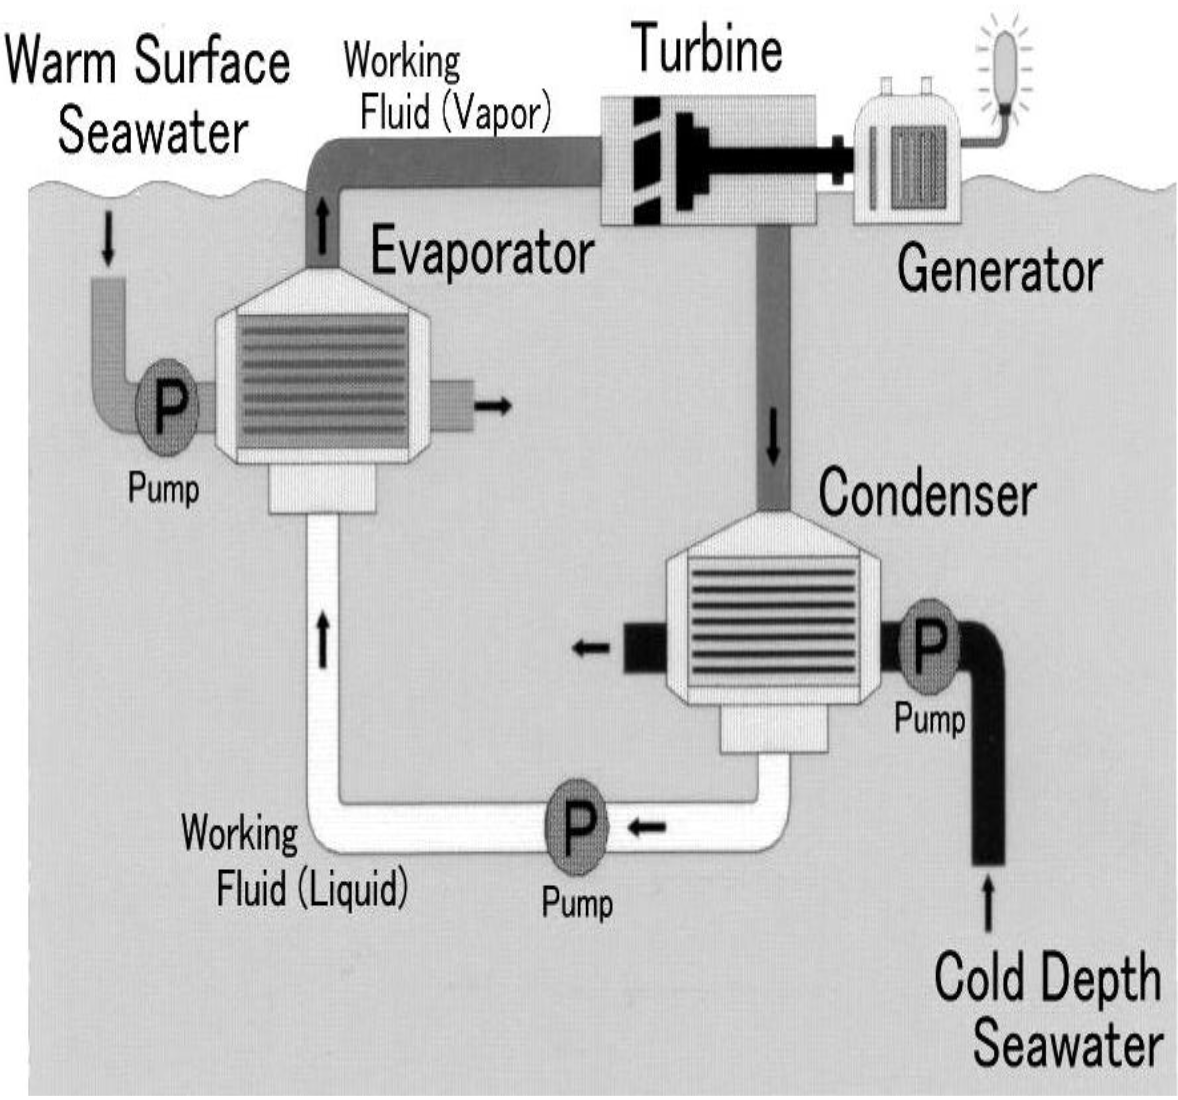
\includegraphics[scale=0.3]{otec}

\section{06. Biofuels}
\begin{itemize}
	\item Plant and animal derived materials that are renewable and carbon neutral
	\item Efficiency of photosynthesis \~0.5\%
	\item Items: Corn, soy, sorghum, sugar cane, waste, sawdust
	\item Low energy content per kilogram and low density -\> bulky and expensive
\end{itemize}
\subsection{Methods of conversion}
\subsubsection{Thermochemical}
\begin{enumerate}
	\item Direct conversion
	\begin{itemize}
		\item Burning solid biomass and production of thermal energy 
	\end{itemize}
	\item Gasification
	\begin{enumerate}
		\item Decompose starting material without oxygen to produce hydrocarbon gases and tar by-product
		\item Heat char again with oxygen to synthesize more gases
	\end{enumerate}
	\begin{itemize}
		\item Advantage: Gaseous fuels mix better than liquid and burns more efficiently and cleanly
		\item Most economically competitive use of biomass
	\end{itemize}
	\item Pyrolysis
	\begin{itemize}
		\item Liquefied by heating in the absence of air
	\end{itemize}
\end{enumerate}
\subsubsection{Biochemical}
\begin{enumerate}
	\item Anaerobic digestion
	\begin{itemize}
		\item Decomposition of organic matter in the absence of air by bacteria
		\item Occurs naturally at 30-60c producing methane for heating, cooking and powering generators
		\item \keyword{biogas}{Methane and C02}
	\end{itemize}
	\item Fermentation
	\begin{itemize}
		\item Using yeast or bacteria to convert to ethanol and CO2
	\end{itemize}
\end{enumerate}
\subsubsection{Extraction}
\begin{itemize}
	\item \keyword{trans esterification}{Reaction with oil using sodium/potassium hydroxide as catalyst to form ethyl/methyl esters (biodiesel)}
\end{itemize}

\subsection{Impact}
\begin{itemize}
	\item Energy security since biomass is more evenly distributed over earth's surface
	\item Rural economic growth
	\item Good and easy storage options
\end{itemize}
\section{07. Geothermal}
\begin{itemize}
	\item Energy extracted from heat stored in the earth
	\item Formation of the planet, radioactive decay of mineral, volcanic activity and from solar energy absorbed by surface
	\item Flowing from the hot core by conduction and convection
	\item Dissipates to atmosphere and space 
	\item Strongest along tectonic plate boundaries
\end{itemize}
\subsection{Methods}
\begin{enumerate}
	\item Borehole heat exchangers
	\begin{itemize}
		\item Heat extraction from ambient rock formation
	\end{itemize}
	\item Hydrothermal systems
	\begin{itemize}
		\item Heat extraction from thermal groundwater
	\end{itemize}
	\item Hot-dry rock
	\begin{itemize}
		\item Water circulation through stimulated fractured rock
	\end{itemize}
\end{enumerate}

\subsection{Sources}
\begin{itemize}
	\item Hot springs
	\begin{itemize}
		\item Gushes of hot water found on land surface
		\item Water vapor emission from cooling molten which rises through rocks to condense at surface
	\end{itemize}
	\item Fumaroles
	\begin{itemize}
		\item Vents from which volcanic gas escapes into the atmosphere
		\item Persistent for decades and centuries
		\item Dangerous gas at around 70-100c
	\end{itemize}
	\item Geysers
	\begin{itemize}
		\item Hot spring erupting periodically ejecting a column of hot water and steam
	\end{itemize}
\end{itemize}

\subsection{Extraction}
\begin{enumerate}
	\item Dry steam system
	\begin{itemize}
		\item 180-225c, 4-8 MPa at 200km/h
		\item Drive steam generator at 1 kWh/6.5kg of steam
		\item Suitable where geothermal steam is not mixed with water
		\item Wells drilled to aquifer and superheated pressurised steam brought to surface at high speeds
		\item Efficiency: 30\%, simplest and most economical technology
	\end{itemize}
	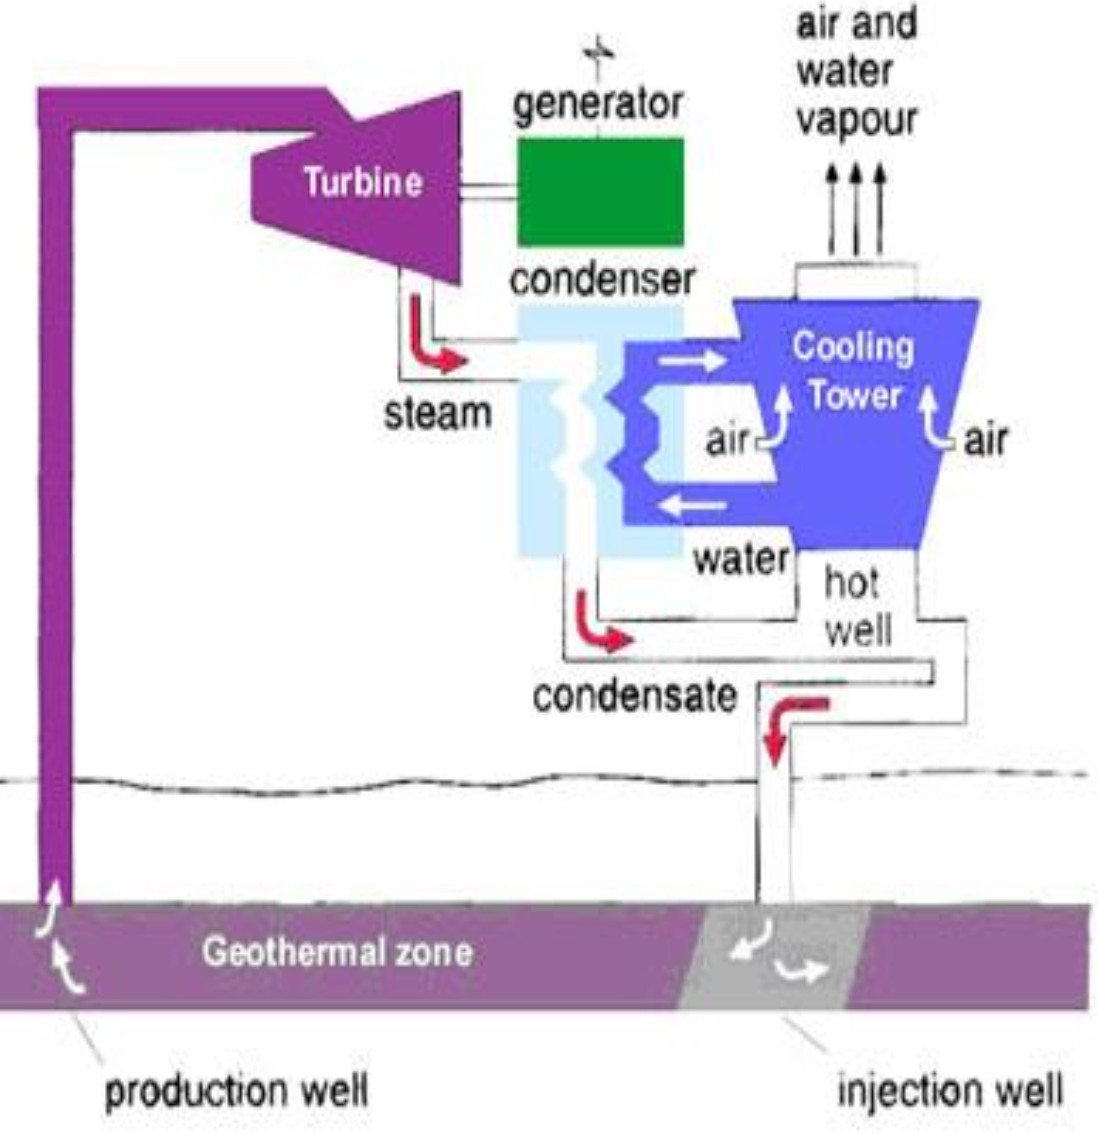
\includegraphics[scale=0.28]{dry-steam}
	\item Flash system
	\begin{itemize}
		\item Steam with water extracted and water flashes to steam when pressure drops suddenly
		\item Steam separated from water and used to drive a turbine
		\item Generates 5-100MW using 6-9 tonnes of steam per hour
		\item Single or double[More efficient but higher cost] flashed systems 
	\end{itemize}
	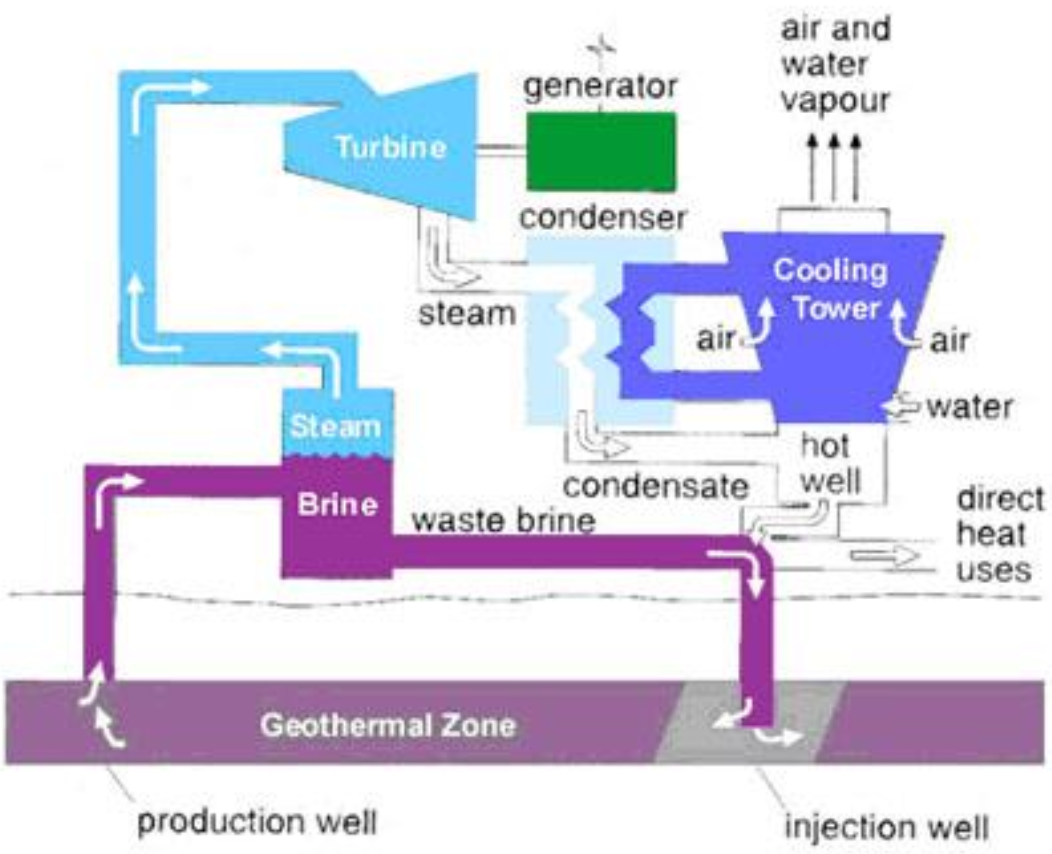
\includegraphics[scale=0.3]{single-flash}\\
	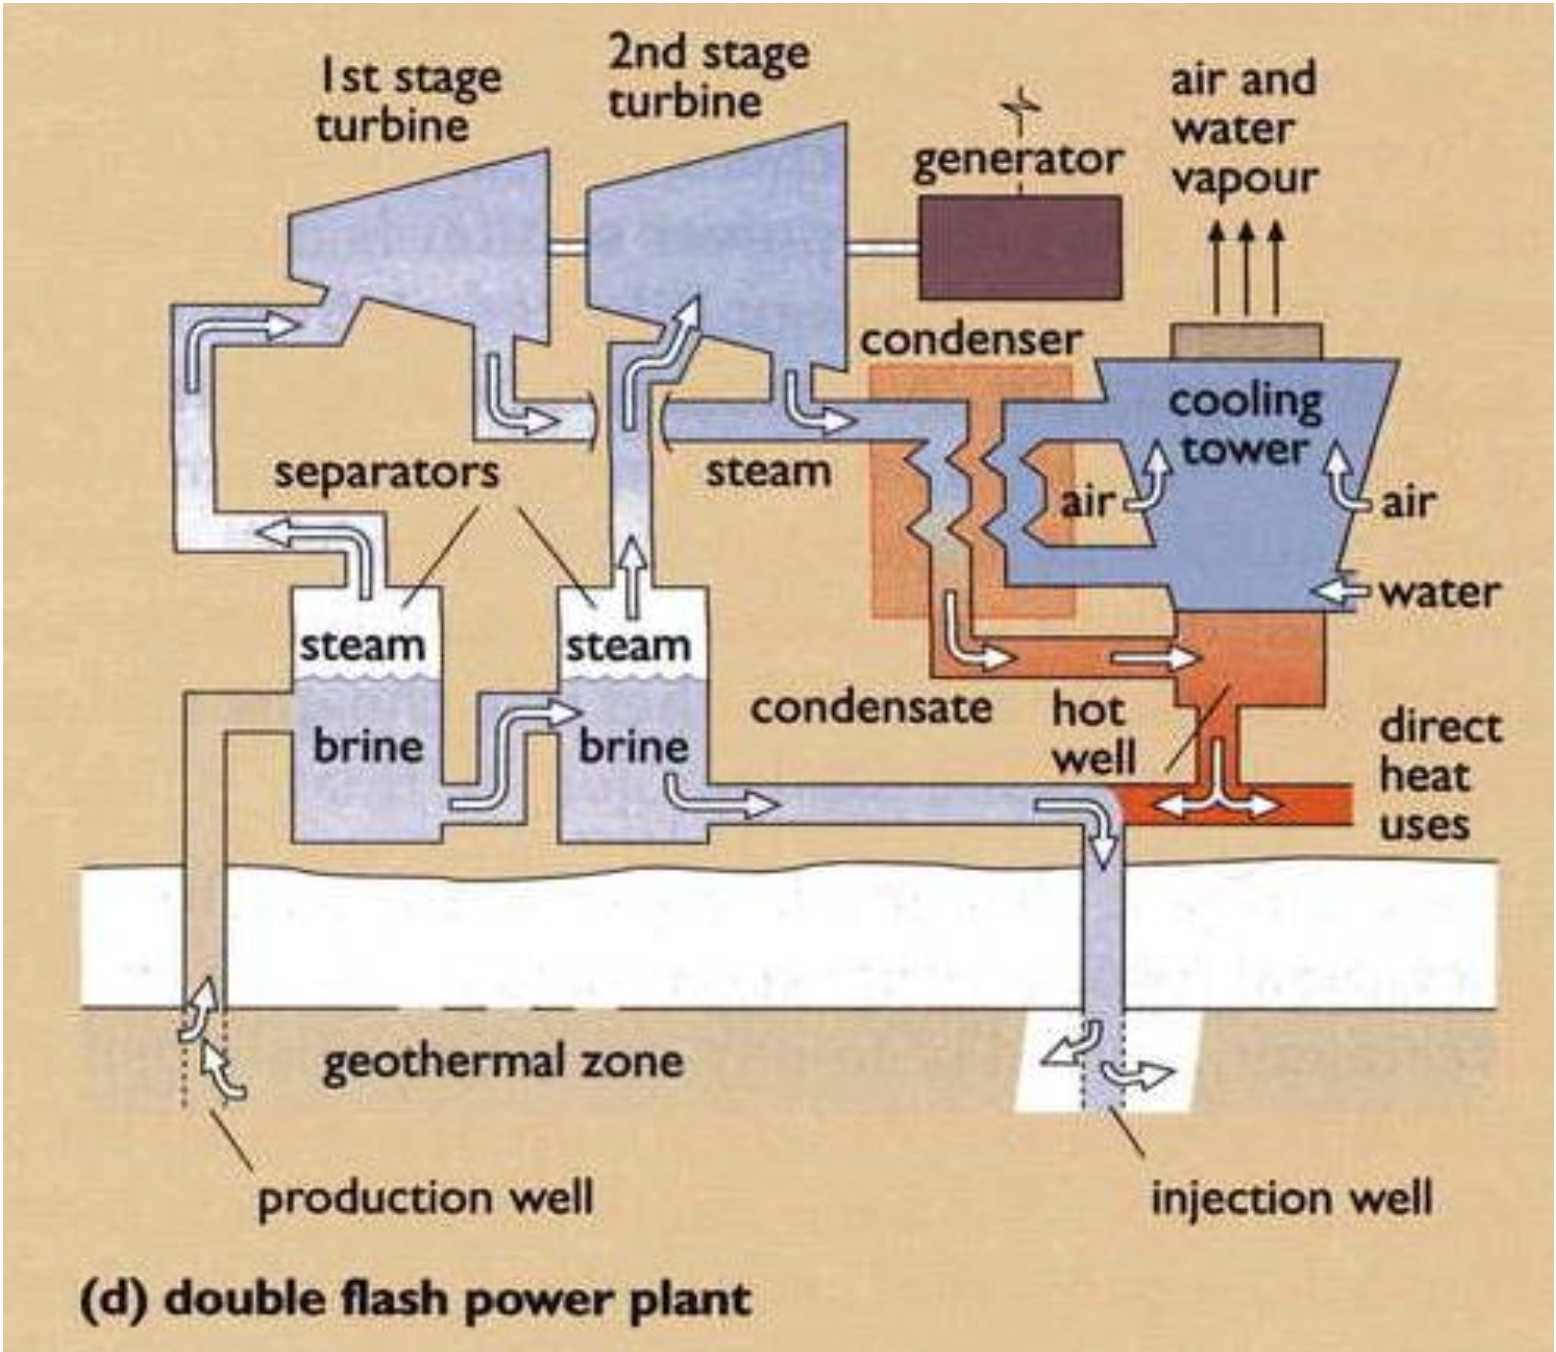
\includegraphics[scale=0.2]{double-flash}
	\item Binary cycle system
	\begin{itemize}
		\item Used for geothermal resource with low temperatures with liquids with low boiling points
		\item Liquids boiled to drive turbine which condenses and recycles continuously
		\item 7-12\% efficient
		\item More expensive but can have higher efficiencies than flash plants
	\end{itemize}
	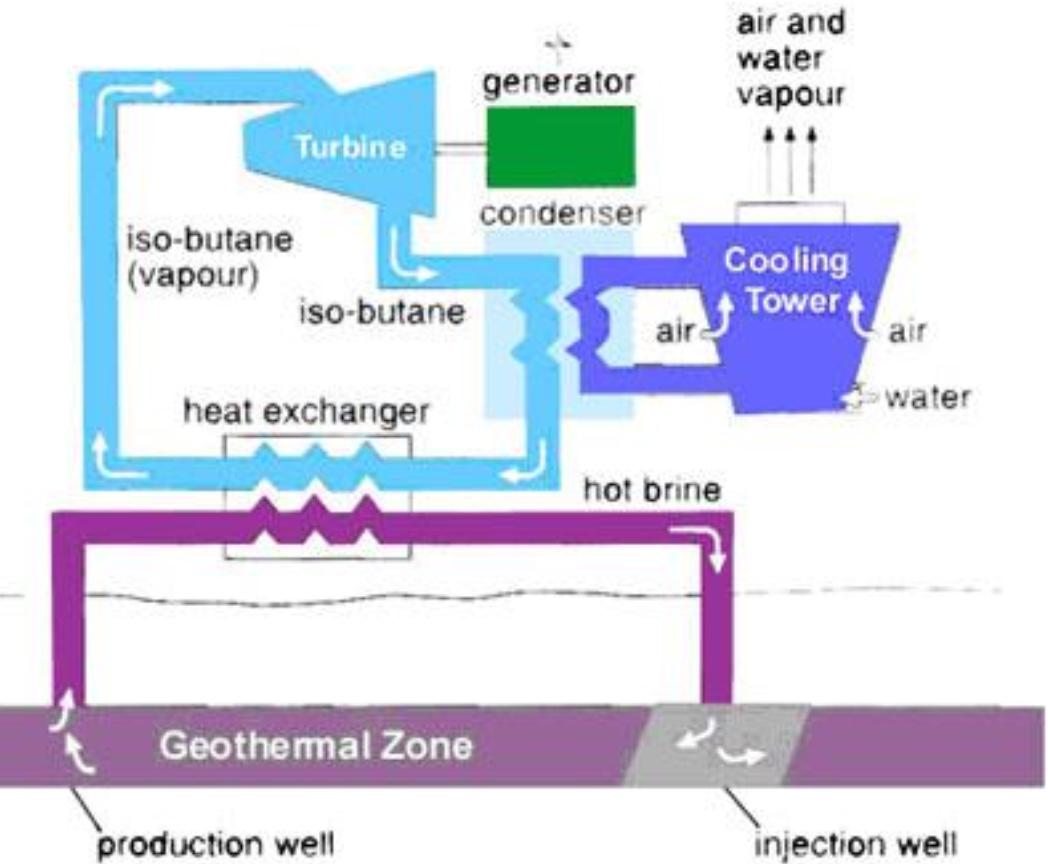
\includegraphics[scale=0.32]{binary-cycle}
	\item Geothermal heat pumps
	\begin{itemize}
		\item Storing and retrieving heat from earth using anti-freeze/water solution circulated in plastic pipe loops 200m into ground
	\end{itemize}
\end{enumerate}

\subsection{Concerns}
\begin{itemize}
	\item Environmental impacts (tremors, \keyword{subsidence}{sinking of ground})
	\item Non-steady state source
	\item High initial capital cost but minimal operating cost
\end{itemize}
\end{multicols*}
\end{document}
